\chapter{Arhitektura i dizajn sustava}
		
	Arhitektura našeg sustava sastoji se od odvojenih backend (Spring Boot) i frontend (React) dijelova. Backend je implementiran pomoću Spring Boot radnog okvira, dok je frontend razvijen korištenjem React biblioteke. 
	\\
	\textbf{Backend (Spring Boot):}
	\\
	\textit{Controller sloj:}
	
	Kontroleri (Controllers) su odgovorni za obradu HTTP zahtjeva i interakciju s korisnicima preko API-ja.
	Svaki kontroler ima metode koje definiraju ponašanje sustava u odgovoru na različite zahtjeve (npr., dohvat podataka, ažuriranje resursa).
	\\
	\textit{Service sloj:}
	
	Servisi (Services) sadrže poslovnu logiku aplikacije.
	Oni obrađuju zahtjeve primljene od kontrolera, vrše potrebne validacije, te komuniciraju s entitetima u bazi podataka.
	Servisi su odvojeni kako bi omogućili ponovnu uporabu koda i jasnu strukturu.
	\\
	\textit{Entity sloj:}
	
	Entiteti predstavljaju objekte koji se pohranjuju u bazi podataka.
	Ovi entiteti često odražavaju strukturu podataka u aplikaciji i pomažu u mapiranju podataka iz baze.
	\\
	\textit{Database sloj:}
	
	Za povezivanje s bazom podataka, koristili smo PostgreSQL.
	JPA (Java Persistence API) može se koristiti za mapiranje objektnih entiteta na relacijsku bazu podataka.
	\\
	\textbf{Frontend (React):}
	\\
	\textit{Components:}
	
	Komponente čine osnovnu građevnu jedinicu React aplikacije.
	Svaka komponenta obavlja određeni dio funkcionalnosti i ima svoje stanje (state) i propertije (props).
	\\
	\textit{API pozivi:}
	
	Komponente koje zahtijevaju podatke s backend-a koriste HTTP zahtjeve prema odgovarajućim API endpointima koristeći
	paketa Axios.
	\\
	\textit{Routing:}
	
	React Router se koristi za omogućavanje rute u aplikaciji, što omogućava navigaciju između različitih dijelova aplikacije.
	\\
	\textit{Styling:}
	
	Za stilizaciju koristimo CSS i CSS-in-JS pristup, gdje stilovi mogu biti integrirani unutar JavaScript datoteka.
	\\
	Ova arhitektura omogućava jasnu odvojenost između frontend i backend dijelova, olakšava održavanje, i omogućuje timsku suradnju s obzirom na to da se razvoj obavlja na odvojenim tehnologijama i dijelovima sustava.
		

		

				
		\section{Baza podataka}
				
				Za bazu podataka koristi se relacijska baza podataka. Svaka tablica ima svoje ime i atribute. Vrste atributa koji se mogu nalaziti u tablici su primarni ključ, strani ključ ili atribut s nekom informacijom vezanom za tablicu. Baza podataka sastoji se od tablica:
		
				\begin{packed_item}
					\item AppUser
					\item ConfirmationToken
					\item StationManager
					\item SearcherInTheField
					\item Action
					\item Station
					\item Animal
					\item PastRoutes
					\item PastLocations
					\item AnimalComment
					\item MapComment
					\item Task
				\end{packed_item}
				
				
		
			\subsection{Opis tablica}
			

				U tablici \textbf{AppUser} pohranjuju se podaci o svim korisnicima: \textit{id, userName, image, firstName, lastName, email, password, appUserRole, locked, enabled}. Primarni ključ je \textit{id}, i nema stranih ključeva. S atributom \textit{id} je u odnosu One-to-One s tablicama \textbf{StationManager} i \textbf{SearcherInTheField} i u odnosu One-to-Many s tablicama \textbf{ConfirmationToken} i \textbf{Action}.

				
				
				\begin{longtblr}[
					label=none,
					entry=none
					]{
						width = \textwidth,
						colspec={|X[6,l]|X[6, l]|X[20, l]|}, 
						rowhead = 1,
					} %definicija širine tablice, širine stupaca, poravnanje i broja redaka naslova tablice
					\hline \SetCell[c=3]{c}{\textbf{AppUser}}	 \\ \hline[3pt]
					\SetCell{LightGreen}id & BIGINT	&  	id korisnika 	\\ \hline
					userName	& VARCHAR &  korisničko ime 	\\ \hline 
					image & BYTEA &  heksadekatski zapis korisničke slike  \\ \hline 
					firstName & VARCHAR	&  ime korisnika  \\ \hline 
					lastName & VARCHAR	&  prezime korisnika  \\ \hline 
					email & VARCHAR	&  email korisnika  \\ \hline 
					password & VARCHAR	&  lozinka korisnika  \\ \hline
					appUserRole & VARCHAR	&  uloga korisnika  \\ \hline 
					locked & BOOLEAN & je li korisnika potvrdio admin \\ \hline
					enabled & BOOLEAN & je li korisnik potvrđen emailom \\ \hline
				\end{longtblr}
				
				U tablici \textbf{ConfirmationToken} pohranjuju se podaci za token za potvrdu poslanu korisniku: \textit{id, token, createdAt, expiresAt, confirmedAt, user}. Svaki token je povezan s korisnikom kojem je poslan preko \textit{user} u koji se sprema id korisnika. Primarni ključ je \textit{id}, a strani ključ je \textit{user}. S atributom \textit{user} je u odnosu Many-to-One s tablicom \textbf{AppUser}.
				
				\begin{longtblr}[
					label=none,
					entry=none
					]{
						width = \textwidth,
						colspec={|X[6,l]|X[6, l]|X[20, l]|}, 
						rowhead = 1,
					} %definicija širine tablice, širine stupaca, poravnanje i broja redaka naslova tablice
					\hline \SetCell[c=3]{c}{\textbf{ConfirmationToken}}	 \\ \hline[3pt]
					\SetCell{LightGreen}id & BIGINT	&  	id tokena 	\\ \hline
					token & VARCHAR & token \\ \hline
					createdAt & TIMESTAMP & vrijeme kada je token stvoren \\ \hline
					expiersAt & TIMESTAMP & vrijeme kada token ističe \\ \hline
					confirmedAt & TIMESTAMP & vrijeme kada je token potvrđen \\ \hline
					\SetCell{LightBlue}user	& BIGINT &  id korisnika kojemu je poslan token \\ \hline  
				\end{longtblr}

				U tablici \textbf{StationManager} pohranjuju se dodatni podaci za voditelja postaje: \textit{stationManagerId, userId, stationId}. Primarni ključ  je \textit{stationManagerId}, te su \textit{userId } i \textit{stationId }  su strani ključevi. S atributom \textit{userId } je u odnosu One-to-One s tablicom \textbf{AppUser}, s atributom \textit{stationManagerId} je u odnosu Many-to-One s tablicom \textbf{Station}.

				
				\begin{longtblr}[
					label=none,
					entry=none
					]{
						width = \textwidth,
						colspec={|X[6,l]|X[6, l]|X[20, l]|}, 
						rowhead = 1,
					} %definicija širine tablice, širine stupaca, poravnanje i broja redaka naslova tablice

					\hline \SetCell[c=3]{c}{\textbf{StationManager}}	 \\ \hline[3pt]
					\SetCell{LightGreen}id & BIGINT	&  	id korisničkog računa voditelja 	\\ \hline
					\SetCell{LightBlue}stationId  & BIGINT	&  	id postaje koju vodi voditelj 	\\ \hline
					\SetCell{LightBlue}userId  & BIGINT	&  id usera	\\ \hline
				\end{longtblr}
			

			U tablici \textbf{SearcherInTheField} primarni ključ je \textit{searcherInTheFieldId}. Strani ključevi su \textit{stationId}, \textit{userId} i \textit{actionId}. S atributom \textit{userId} je u odnosu One-to-One s tablicom \textbf{AppUser}, s atributom \textit{stationId} je u odnosu Many-to-One s tablicom \textbf{Station}, s atributom \textit{actionId} je u odnosu Many-to-One s tablicom \textbf{Action}.

			
				\begin{longtblr}[
					label=none,
					entry=none
					]{
						width = \textwidth,
						colspec={|X[10,l]|X[6, l]|X[20, l]|}, 
						rowhead = 1,
					} %definicija širine tablice, širine stupaca, poravnanje i broja redaka naslova tablice
					\hline \SetCell[c=3]{c}{\textbf{SearcherInTheField}}	 \\ \hline[3pt]
					\SetCell{LightGreen}searcherInTheFieldId & BIGINT	&  	id korisničkog računa tragača 	\\ \hline
					\SetCell{LightBlue}stationId & BIGINT	&  	id postaje kojoj pripada 	\\ \hline
					\SetCell{LightBlue} userId  & BIGINT	&  id usera	\\ \hline
					 qualification	& VARCHAR & osposobljenosti tragača 	\\ \hline  
					 currentPosition & JSON &  trenutna pozicija tragača	\\ \hline 
					\SetCell{LightBlue} actionId  & BIGINT	&  id akcije na kojoj tragač sudjeluje	\\ \hline
				\end{longtblr}
			

			U tablici \textbf{Action} pohranjuju se podaci vezani uz određenu akciju. Primarni ključ je \textit{actionId}, a strani ključ je \textit{appUserId}. S atributom \textit{appUserId} je u odnosu Many-to-One s tablicom \textbf{AppUser} i s atributom \textit{stationId} je u odnosu One-to-One s tablicom \textbf{Station}.


			
			\begin{longtblr}[
				label=none,
				entry=none
				]{
					width = \textwidth,
					colspec={|X[8,l]|X[6, l]|X[20, l]|}, 
					rowhead = 1,
				} %definicija širine tablice, širine stupaca, poravnanje i broja redaka naslova tablice
				
				\hline \SetCell[c=3]{c}{\textbf{Action}}	 \\ \hline[3pt]
				\SetCell{LightGreen}  actionId & BIGINT	&  	id akcije 	\\ \hline
				\SetCell{LightBlue}appUserId & BIGINT	&  	id korisnika (istraživača) koji je započeo akciju 	\\ \hline
				\SetCell{LightBlue} stationId & BIGINT	& id postaje kojoj se posalo zahtjev za tragačima \\ \hline
				actionName	& TEXT &  naziv akcije 	\\ \hline
				actionType & TEXT &  tip akcije	\\ \hline  
				locationName & TEXT &  ime lokacije na kojoj se odvija akcija (npr. Biokovo)	\\ \hline 
				mapViewCriteria & JSON & odabrani kriteriji (od strane istraživača) za prikaz životinja na mapi \\ \hline
				qualificationsJson & JSON & popis traženih kvalifikacija tragača na akciji \\ \hline
			\end{longtblr}
			

			U tablici \textbf{Station} pohranjuju se podaci vezani uz postaju. Primarni ključ je \textit{stationId}. Strani ključ je \textit{stationId}. S atributom \textit{stationId} je u odnosu Many-to-One s tablicom \textbf{Station}.
			
			\begin{longtblr}[
				label=none,
				entry=none
				]{
					width = \textwidth,
					colspec={|X[8,l]|X[6, l]|X[20, l]|}, 
					rowhead = 1,
				} %definicija širine tablice, širine stupaca, poravnanje i broja redaka naslova tablice

				\hline \SetCell[c=3]{c}{\textbf{Station}}	 \\ \hline[3pt]
				\SetCell{LightGreen}stationId & BIGINT	&  	id postaje 	\\ \hline
				stationName & VARCHAR & ime postaje \\ \hline
				coordinatesJson & JSON & popis koordinata postaje te koordinata za prikaz područje pokrivanja za određeno osposobljenje \\ \hline
			\end{longtblr}
			
			U tablici \textbf{Animal} o svim životinjama za određenu postaju. Primarni ključ je \textit{animalId} nema stranih ključeva. S atributom \textit{id} je u odnosu One-to-Many s tablicom \textbf{Location}.

			\begin{longtblr}[
				label=none,
				entry=none
				]{
					width = \textwidth,
					colspec={|X[7,l]|X[6, l]|X[20, l]|}, 
					rowhead = 1,
				} %definicija širine tablice, širine stupaca, poravnanje i broja redaka naslova tablice

				\hline \SetCell[c=3]{c}{\textbf{Animal}}	 \\ \hline[3pt]
				\SetCell{LightGreen} animalId & BIGINT	&  	id životinje 	\\ \hline
				name & VARCHAR & ime životinje \\ \hline
				breed & VARCHAR & vrsta životinje \\ \hline
				description & VARCHAR & opis životinje \\ \hline
				image & BYTEA & slika životinje \\ \hline
				currentPosition & JSON & trenutna pozicija životinje\\ \hline
				\SetCell{LightBlue}stationId & BIGINT	&  id postaje, odn. područja (npr. postaja Biokovo) kojoj životinja pripada \\ \hline
			\end{longtblr}
			

			U tablici \textbf{PastRoutes} pohranjuju se podaci o svim prijašnjim rutama kojima je istraživač prošao na određenoj akciji. Primarni ključ je \textit{pastRoutesId}, a strani ključevi su \textit{actionId} i \textit{searcherId}. S atributom \textit{actionId} je u odnosu Many-to-One s tablicom \textbf{Action}, a s atributom \textit{searcherId} je u odnosu Many-to-One s tablicom \textbf{SearcherInTheField} .

			\begin{longtblr}[
				label=none,
				entry=none
				]{
					width = \textwidth,
					colspec={|X[8,l]|X[6, l]|X[20, l]|}, 
					rowhead = 1,
				} %definicija širine tablice, širine stupaca, poravnanje i broja redaka naslova tablice

				\hline \SetCell[c=3]{c}{\textbf{PastRoutes}}	 \\ \hline[3pt]
				\SetCell{LightGreen}pastRoutesId & BIGINT & id rute \\ \hline
				routeWaypoints & JSON & koordinate rute\\ \hline
				\SetCell{LightBlue}actionId & BIGINT	&  id akcije na kojoj je istraživač prošo tom rutom \\ \hline
				\SetCell{LightBlue}searcherId & BIGINT	&  id istraživača čija je ruta zabilježena  \\ \hline
				
			\end{longtblr}
			
			U tablici \textbf{PastLocations} pohranjuju se podaci o svim prijašnjim lokacijama životinja ili istraživača na određenoj akciji. Primarni ključ je \textit{pastLocationId}, a strani ključevi su \textit{actionId}, \textit{animalId} i \textit{searcherId}. S atributom \textit{actionId} je u odnosu Many-to-One s tablicom \textbf{Action}, s atributom \textit{animalId} je u odnosu Many-to-One s tablicom \textbf{Animal}, a s atributom \textit{searcherId} je u odnosu Many-to-One s tablicom \textbf{SearcherInTheField} .
			
			\begin{longtblr}[
				label=none,
				entry=none
				]{
					width = \textwidth,
					colspec={|X[9,l]|X[6, l]|X[20, l]|}, 
					rowhead = 1,
				} %definicija širine tablice, širine stupaca, poravnanje i broja redaka naslova tablice
				
				\hline \SetCell[c=3]{c}{\textbf{PastLocations}}	 \\ \hline[3pt]
				\SetCell{LightGreen}pastLocationId & BIGINT & id lokacije \\ \hline
				positionCoordinates & JSON & koordinate lokacije\\ \hline
				\SetCell{LightBlue}actionId & BIGINT	&  id akcije tokom koje je zabilježena lokacija \\ \hline
				\SetCell{LightBlue}searcherId & BIGINT	&  id istraživača čija je lokacija zabilježenja  \\ \hline
				\SetCell{LightBlue}animalId & BIGINT	&  id životinje čija je prijašnja lokacija zabilježenja  \\ \hline
				
			\end{longtblr}		
			
			U tablici \textbf{AnimalComment} pohranjuju se svi komentari koji su ostavljeni životinji na određenoj akciji. Primarni ključ je \textit{animalCommentId}, a strani ključevi su \textit{actionId} i \textit{animalId}. S atributom \textit{actionId} je u odnosu Many-to-One s tablicom \textbf{Action}, te s atributom \textit{animalId} je u odnosu Many-to-One s tablicom \textbf{Animal}.
			
			\begin{longtblr}[
				label=none,
				entry=none
				]{
					width = \textwidth,
					colspec={|X[9,l]|X[6, l]|X[20, l]|}, 
					rowhead = 1,
				} %definicija širine tablice, širine stupaca, poravnanje i broja redaka naslova tablice
				
				\hline \SetCell[c=3]{c}{\textbf{AnimalComment}}	 \\ \hline[3pt]
				\SetCell{LightGreen}animalCommentId & BIGINT & id komentara \\ \hline
				comment & VARCHAR & komentar ostavljen životinji\\ \hline
				userName & VARCHAR & korisničko ime korisnika koji je ostavio komentar životinji lokacije\\ \hline
				\SetCell{LightBlue}actionId & BIGINT	&  id akcije tokom koje je zabilježena lokacija \\ \hline
				\SetCell{LightBlue}animalId & BIGINT	&  id životinje čija je prijašnja lokacija zabilježenja  \\ \hline
			\end{longtblr}
			
			U tablici \textbf{MapComment} pohranjuju se svi komentari koji su ostavljeni na mapi na određenoj akciji. Primarni ključ je \textit{mapCommentId}, a strani ključ je \textit{actionId}. S atributom \textit{actionId} je u odnosu Many-to-One s tablicom \textbf{Action}.
			
			\begin{longtblr}[
				label=none,
				entry=none
				]{
					width = \textwidth,
					colspec={|X[9,l]|X[6, l]|X[20, l]|}, 
					rowhead = 1,
				} %definicija širine tablice, širine stupaca, poravnanje i broja redaka naslova tablice
				
				\hline \SetCell[c=3]{c}{\textbf{MapComment}}	 \\ \hline[3pt]
				\SetCell{LightGreen}mapCommentId & BIGINT & id komentara \\ \hline
				comment & VARCHAR & komentar ostavljen životinji\\ \hline
				userName & VARCHAR & korisničko ime korisnika koji je ostavio komentar životinji lokacije\\ \hline
				positionCoordinates & JSON & koordinate lokacije gdje je na mapi ostavljen komentar\\ \hline
				\SetCell{LightBlue}actionId & BIGINT	&  id akcije tokom koje je zabilježena lokacija \\ \hline
			\end{longtblr}
			
			U tablici \textbf{Task} pohranjuju se podaci zadataka koji su dodjeljeni tragaču na određenoj akciji. Primarni ključ je \textit{taskId}, strani ključevi su \textit{actionId} i \textit{searcher}. S atributom \textit{actionId} je u odnosu Many-to-One s tablicom \textbf{Action}, a s atributom \textit{searcherId} je u odnosu Many-to-One s tablicom \textbf{SearcherInTheField}.
			
			\begin{longtblr}[
				label=none,
				entry=none
				]{
					width = \textwidth,
					colspec={|X[9,l]|X[6, l]|X[20, l]|}, 
					rowhead = 1,
				} %definicija širine tablice, širine stupaca, poravnanje i broja redaka naslova tablice
				
				\hline \SetCell[c=3]{c}{\textbf{Task}}	 \\ \hline[3pt]
				\SetCell{LightGreen}taskId & BIGINT & id zadatka \\ \hline
				taskComment	& VARCHAR &  komentar za zadatak od strane istraživača	\\ \hline 
				taskToDo	& VARCHAR &  opis  što tragač mora napraviti 	\\ \hline 
				completed & BOOLEAN & je li zadatak završen ili ne \\ \hline
				routeWaypoints & JSON & koordinate rute koju tragač treba proći na zadatku\\ \hline
				\SetCell{LightBlue}searcherId & BIGINT	&  id istraživača čija je lokacija zabilježenja  \\ \hline
				\SetCell{LightBlue}actionId & BIGINT	&  	id akcije kojoj pripada zahtjev 	\\ \hline
			\end{longtblr}
			
			\subsection{Dijagram baze podataka}
				\begin{figure}[H]
					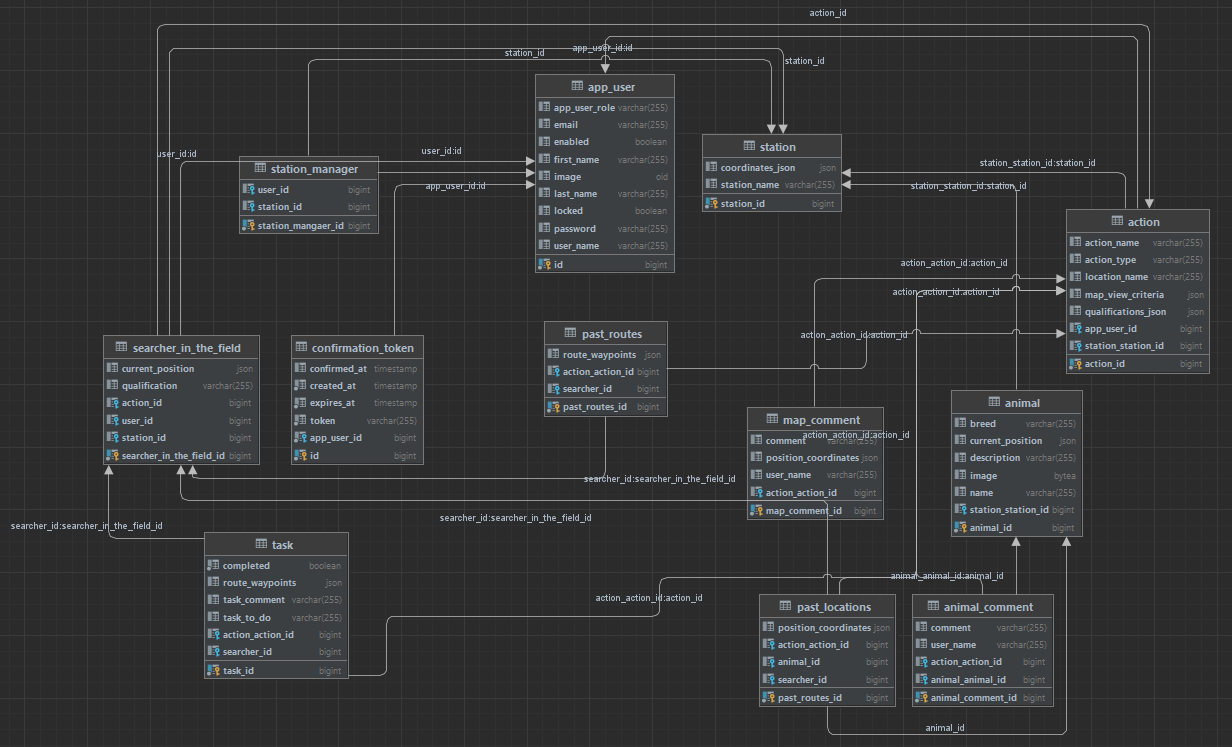
\includegraphics[scale=0.6]{dijagrami/dijagramBaza.png}
					\centering
					\caption{Dijagram baze podataka}
					\label{fig:promjene}
				\end{figure}
			\eject
			
			
		\section{Dijagram razreda}
		Dijagram razreda podijeljen je zbog bolje preglednosti na tri dijela: Controllers, Models i DTO. Prikazane su veze koje ostvaruju razredi unutar istog dijela dijagrama, a odnosi između razreda u različitim dijelovima mogu se zaključiti iz tipova atributa. Metode korištene u Controller razredima vraćaju \textit{ResponseEntity}, koji predstavlja HTTP odgovor, ili samo kod odgovora HTTP-a. U svom radu koriste objekte za prijenos podataka (DTO) i ostvaruju komunikaciju s klijentskom stranom.
			
			\begin{figure}[H]
				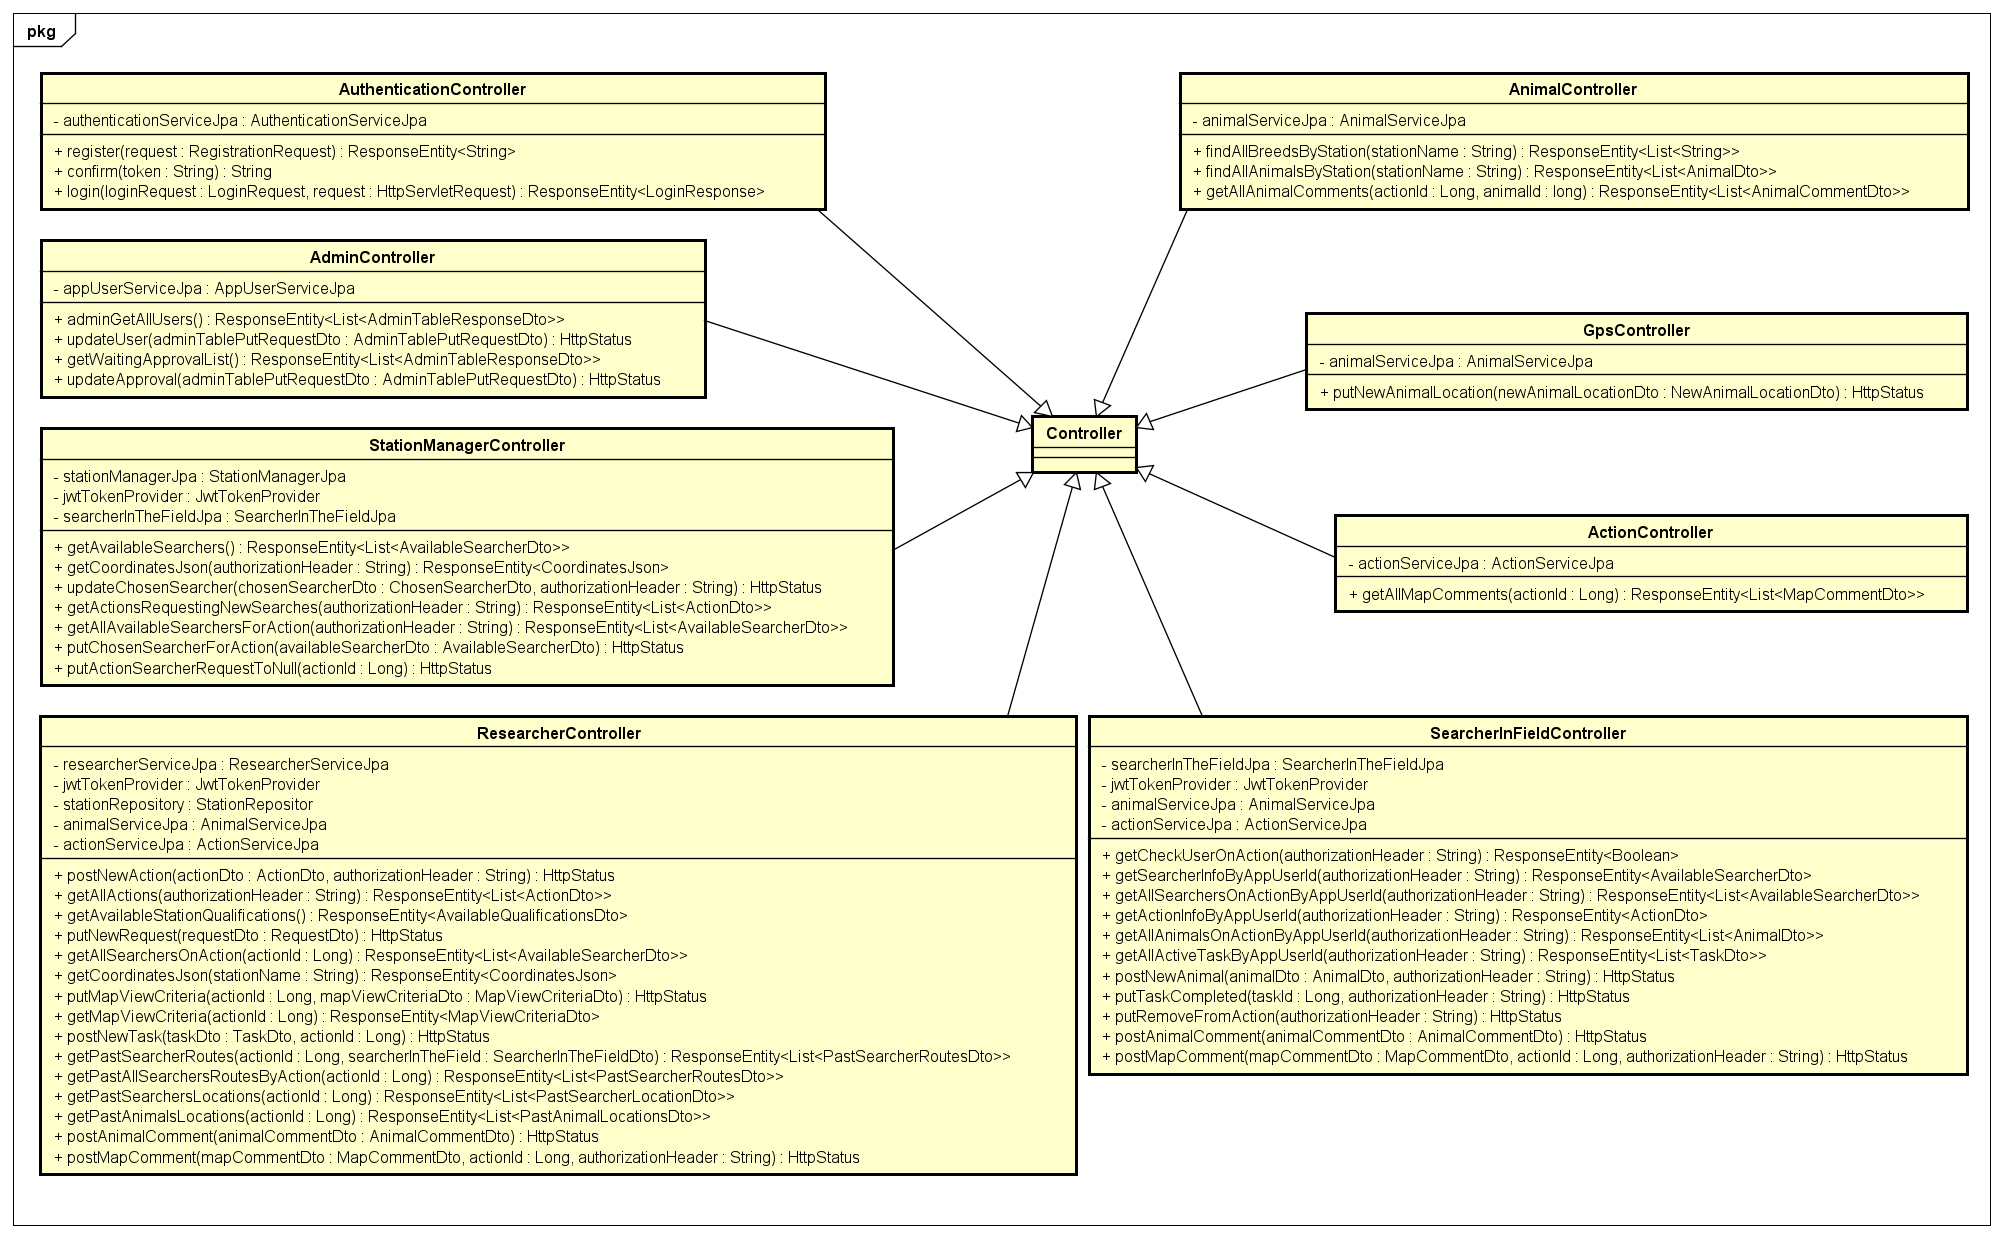
\includegraphics[scale=0.3]{dijagrami/Controllers.png} 
				\centering
				\caption{Dijagram razreda - dio Controllers}
				\label{fig:promjene}
			\end{figure}
			
			\begin{figure}[H]
				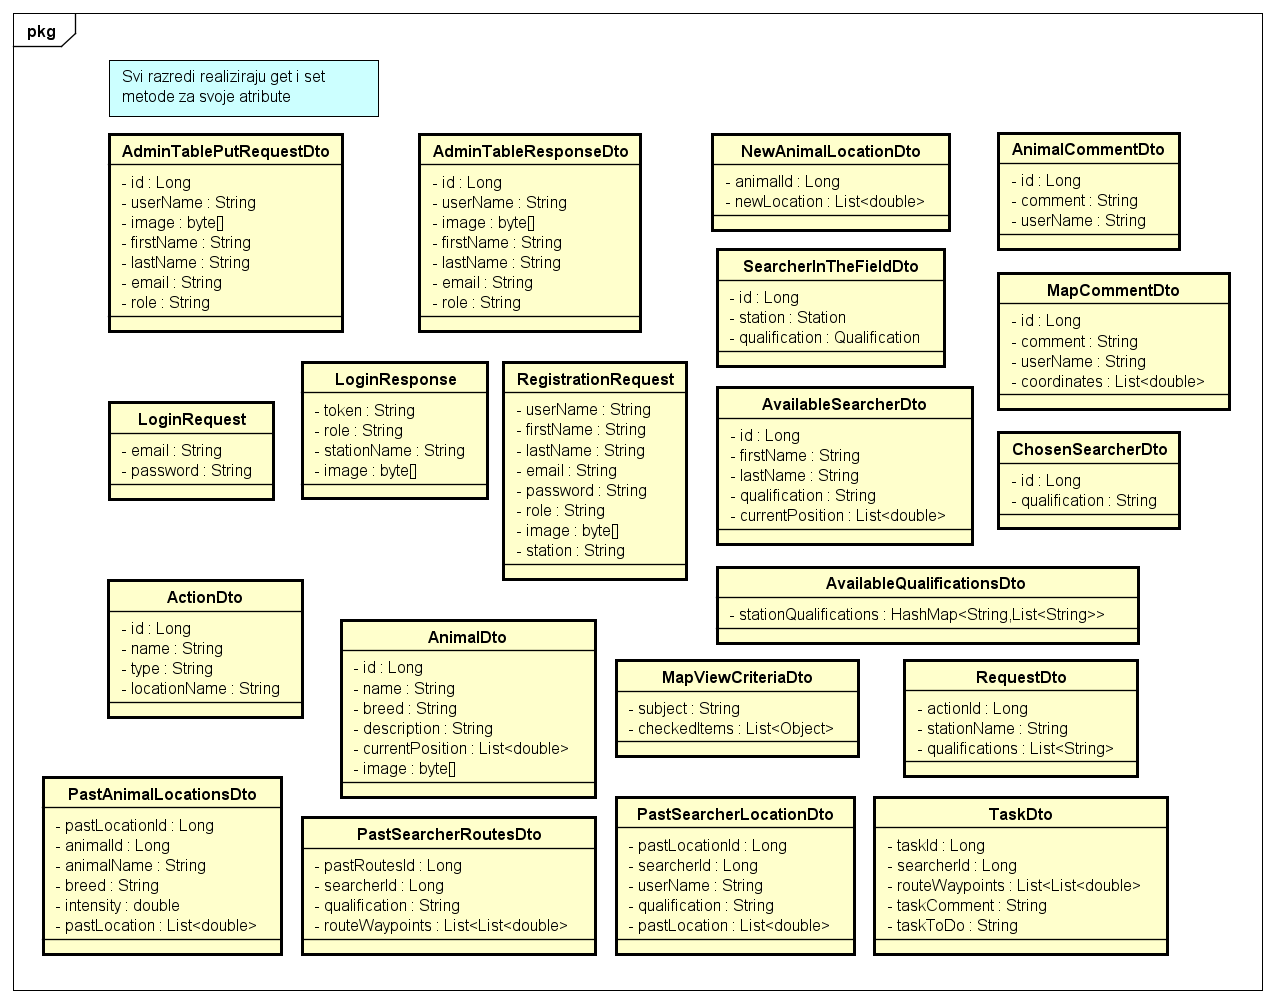
\includegraphics[scale=0.5]{dijagrami/DTO.png} 
				\centering
				\caption{Dijagram razreda - dio DTO}
				\label{fig:promjene}
			\end{figure}
			
			\begin{figure}[H]
				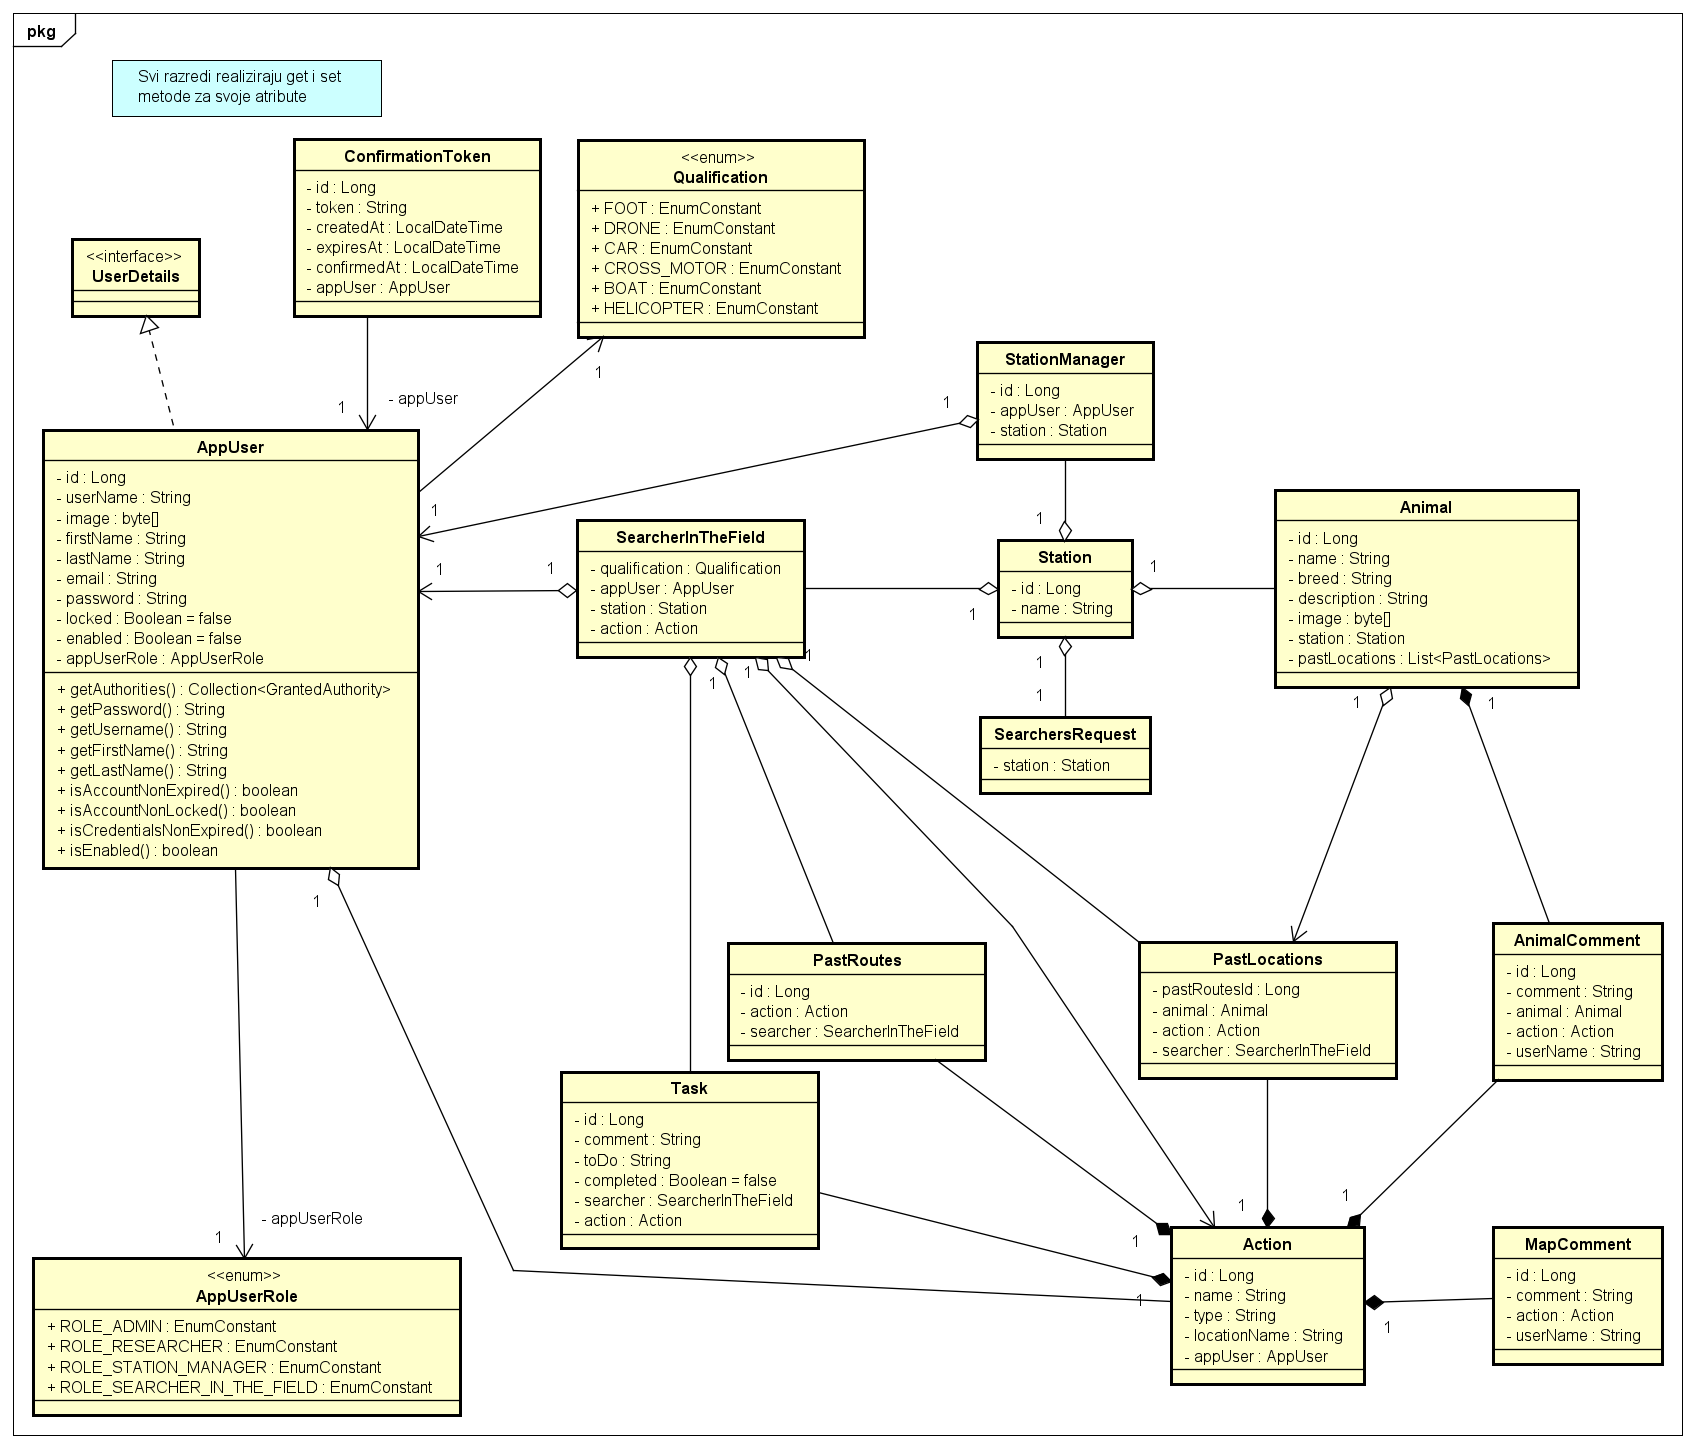
\includegraphics[scale=0.4]{dijagrami/Model.png} 
				\centering
				\caption{Dijagram razreda - dio Models}
				\label{fig:promjene}
			\end{figure}
			
			
			\eject
		
		\section{Dijagram stanja}
			
			
			Dijagrami stanja prikazuju kako sustav prelazi iz jednog stanja u drugo kao odgovor na događaje. Prijavljenom korisniku, u ovom slučaju istraživaču, prikazuje se početna stranica s aktivnim akcijama i nekoliko opcija: stvaranje nove akcije, prikaz interaktivne karte i slanje zahtjeva za tragačima. Nakon odabira opcije stvaranja nove akcije, korisniku se prikazuje forma za unos podataka o akciji. Spremanjem akcije korisnik ponovno vidi početnu stranicu. Odabirom slanja zahtjeva za tragačima za neku od akcija, istraživaču se prikazuje forma za unos detalja o zahtjevu. U slučaju da nema slobodnih tragača, sustav obavijesti korisnika i čeka na idući zahtjev. Odabirom opcije ,,Više detalja“, istraživaču se prikaže interaktivna karta koju može uređivati po želji. Ako je odabran prikaz tragača na karti, korisnik može nekome od njih dodijeliti zadatak. Zatim ima opciju unosa komentara na zadatak. Također, istraživač može ostaviti komentar na samoj karti.
			
			\begin{figure}[H]
				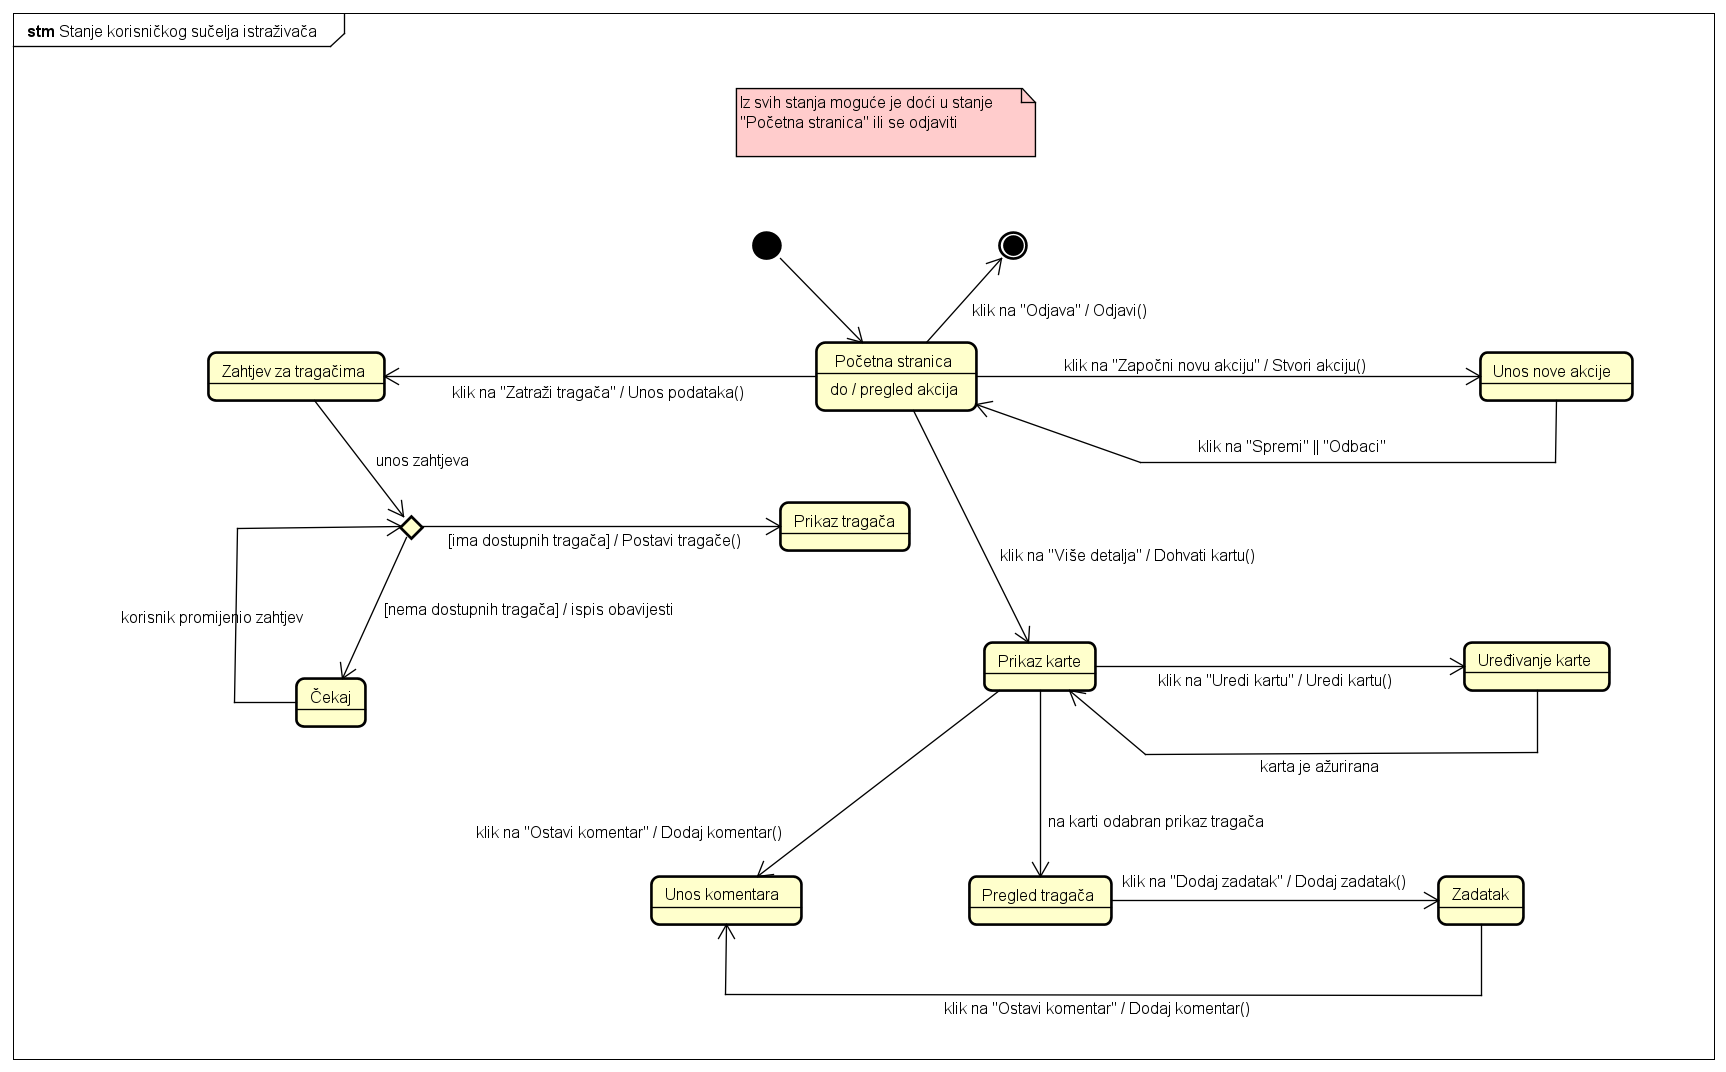
\includegraphics[scale=0.3]{dijagrami/DijStanja.png} 
				\centering
				\caption{Dijagram stanja}
				\label{fig:promjene}
			\end{figure}
			
			
			\eject 
		
		\section{Dijagram aktivnosti}
			
			Dijagrami aktivnosti upotrebljavaju se za modeliranje dinamičkog ponašanja sustava. Izvođenje aktivnosti prikazano je kroz niz akcija koje čine upravljačke tokove i tokove objekata. Prikazan je proces stvaranja nove akcije. Aktivnost započinje prijavom istraživača u sustav. Nakon uspješne prijave, istraživaču se prikazuje početna stranica. Odabirom opcije za stvaranje nove akcije aplikacija prikazuje formu za unos podataka o akciji. Istraživač unosi podatke o akciji, a sustav ih pohranjuje u bazu podataka. Zatim istraživač šalje zahtjev za tragačima, a aplikacija prikazuje formu za unos detalja o zahtjevu. Aplikacija prosljeđuje zahtjev voditelju postaje koji dodjeljuje tragače akciji (pretpostavlja se da ima dostupnih tragača). Popis tragača se pohranjuje u bazu i prikazuje u aplikaciji. Na zahtjev za dodjeljivanje zadatka nekom od tragača prikazuje se forma za unos zadatka. Zadatak se sprema u bazu podataka, a istraživač unosi komentar o zadatku. Nakon završetka unosa svih podataka o akciji aplikacija prikazuje poruku da su svi podaci spremljeni i aktivnost završava.
			
			\begin{figure}[H]
				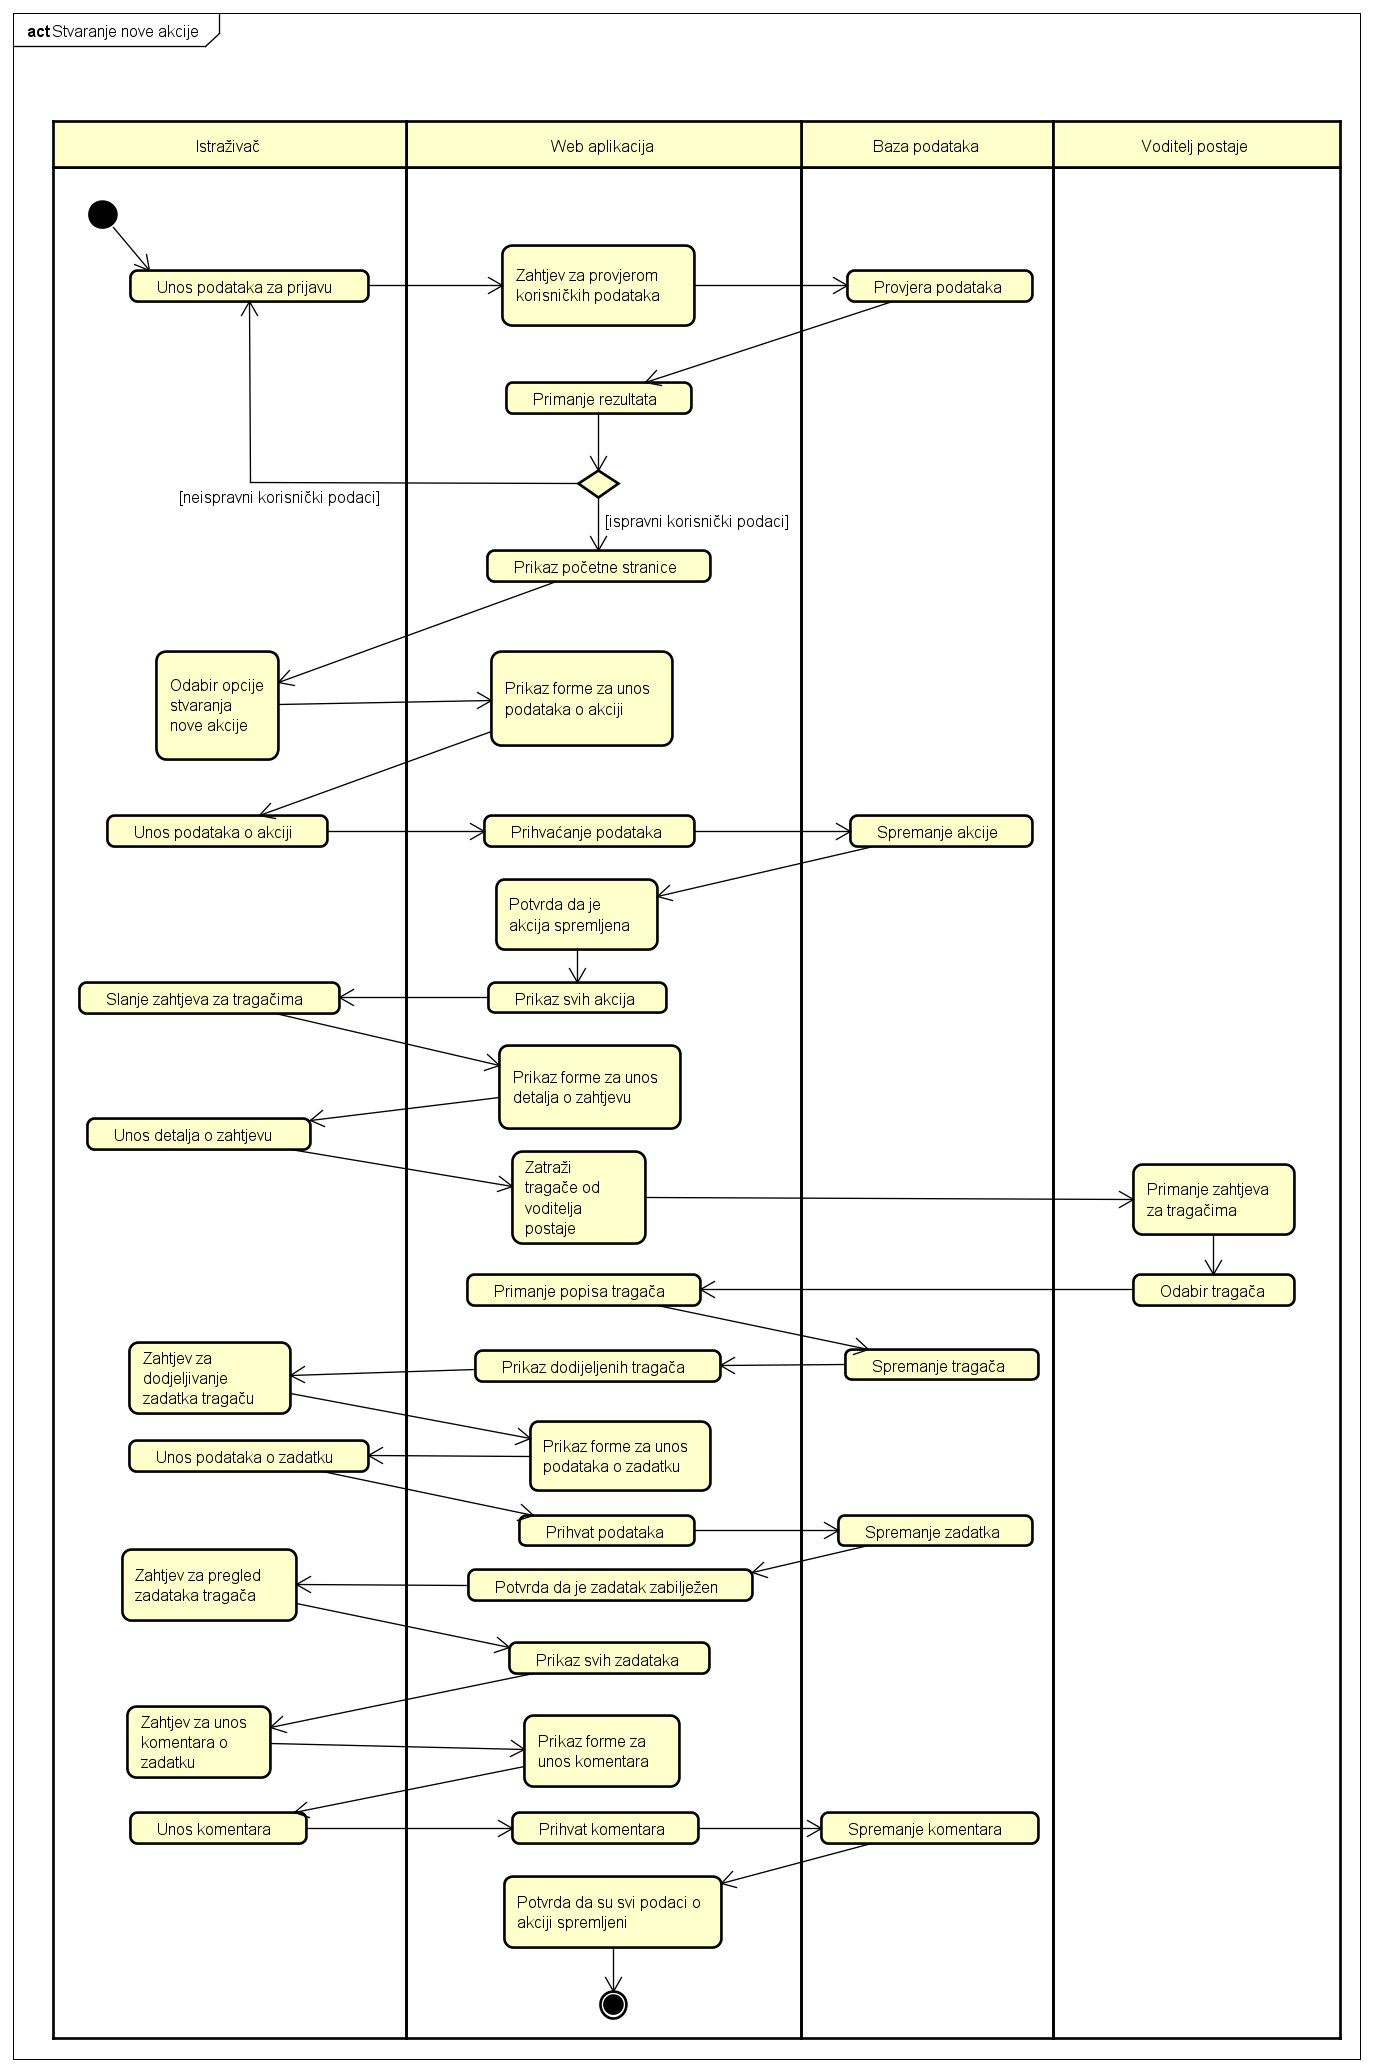
\includegraphics[scale=0.4]{dijagrami/DijAktivnosti.png} 
				\centering
				\caption{Dijagram aktivnosti}
				\label{fig:promjene}
			\end{figure}
			
			\eject
		\section{Dijagram komponenti}
		
			 Dijagram komponenti prikazuje komponente u sustavu i njihovu organizaciju. Sustav se sastoji od tri glavne komponente: \textbf{Frontend web aplikacije}, \textbf{Backend web aplikacije} i \textbf{Baza podataka}. \textbf{Frontend web aplikacije} sastoji se od manjih komponenti: \textbf{ApiService.js, index.js, Admin, Assets, General, Login, Manager, Register, Researcher, Searcher}. Komponenta \textbf{ApiService.js} služi za komunikaciju s backendom pomoću HTTP metoda \textit{get, post, put, delete}. Komponente \textbf{Admin, Assets, General, Login, Manager, Register, Researcher, Searcher} su skupovi react komponenti koji služe za prikaz za određenu svrhu. Npr. \textbf{Admin} ima komponente koje se prikazuju samo za admina, a \textbf{Manager} ima komponente koje se pokazuju samo za voditelja postaje. \textbf{Backend web aplikacije} sastoji se od komponenti \textbf{Controller, Service, Mapper, DTO, Repository}. \textbf{Controller} prima i odgovara na HTTP metode i poziva usluge u komponenti \textbf{Service}. Komponenta \textbf{Service} obavlja funkcije aplikacije, npr. registracija korisnika, dodavanje komentara, stvaranje postaje itd. Komponenta \textbf{Repository} služi za komunikaciju s \textbf{Bazom podataka}. \textbf{DTO} sadrži objekte s podacima koji se koriste u aplikaciji. \textbf{Mapper} služi za pretvorbu objekata iz \textbf{DTO} u normalne objekte, npr. pretvorbu AnimalDto u Animal.
			 
			 
			 \begin{figure}[H]
			 	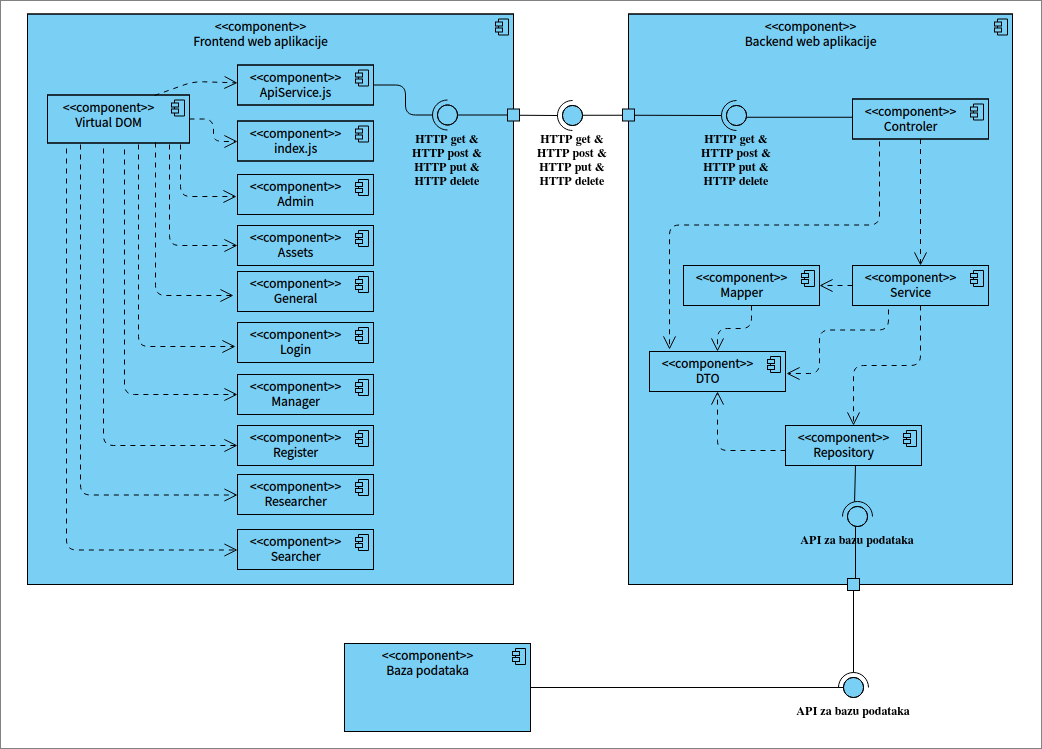
\includegraphics[scale=0.45]{dijagrami/dijagram_komponenti2.png}
			 	\centering
			 	\caption{Dijagram komponenti}
			 	\label{fig:promjene}
			 \end{figure}